\documentclass{article}
\usepackage[final,nonatbib]{neurips_2019}
\usepackage[utf8]{inputenc}
\usepackage[T1]{fontenc}
\usepackage{amsmath,amssymb,booktabs,graphicx,microtype,float}
\usepackage[hidelinks]{hyperref}
\hypersetup{pdftitle={Do Consistent Learned Forces Find the Right Molecular Shape?},pdfauthor={Shedrack Eze; Olufunke Abodunrin; Emmanuel Aaron; Muhammed Idris}}
\makeatletter
\renewcommand{\@noticestring}{11-785 Introduction to Deep Learning, Fall 2026. Group 9 midsemester working draft, 18 October 2026.}
\makeatother
\title{Do Consistent Learned Forces Find the Right Molecular Shape?}
\author{Shedrack Eze (seze) \quad Olufunke Abodunrin (oabodunr)\\
\textbf{Emmanuel Aaron (eaaron) \quad Muhammed Idris (midris)}\\
Carnegie Mellon University \quad Group 9, Path 3}
\newcommand{\forceunit}{\mathrm{eV}/\text{\AA}}
\begin{document}
\maketitle
\begin{abstract}
A molecular force model can make accurate predictions on stored examples yet lead a molecule to the wrong shape when its forces are followed. We test whether training directly predicted forces to agree with a learned energy improves correct-shape recovery at comparable force error. On aspirin from Landscape17, we implemented energy-derived, direct and consistency-trained E3x models and an independently scored MACE reference. Two-seed validation force errors are comparable for direct prediction and consistency strength 0.1. Every evaluated model, including the energy baseline, recovers zero of ten branch references, even though all target minima appear in training. This pilot therefore cannot distinguish the methods. Follow-up checks find excessive predicted forces at reference geometries and extreme accepted coordinate steps. The hypothesis remains unsupported under this procedure; its broader validity is unresolved.
\end{abstract}
\section{Motivation and objective}
Quantum-chemistry energy and force calculations are expensive to repeat during simulation. Learned interatomic potentials offer a cheaper approximation, whose usefulness depends on the motion it produces as well as stored-example accuracy.

Energy-derived models obtain forces from one learned scalar energy. Direct models predict vectors, which may be cheaper but need not follow an energy surface. We ask whether encouraging their agreement improves reference-conformation recovery from withheld pathways at comparable force error and cost. Recovery requires force convergence and structural agreement; a stopped direct-force field need not define an energy minimum.
\section{Related work}
Landscape17 provides stationary points and descent pathways for evaluating learned potential-energy landscapes \cite{landscape}. Its results motivate measuring structural recovery alongside predictive accuracy; our withheld-connection study is not a reproduction of its complete kinetic-network benchmark. Bigi et al. identify difficulties with nonconservative forces in geometry optimization and dynamics \cite{bigi}. This motivates separating force convergence from structural success.

We implement a common equivariant backbone with E3x \cite{e3x}, and MACE as an established external predictive reference \cite{mace}. Physics-informed losses have already been studied for interatomic potentials, including conservative-force constraints \cite{takamoto}. Our contribution is the controlled error--cost--recovery comparison and its failure analysis, rather than a claim that energy--force consistency training is new.
\section{Data, models and evaluation}
\subsection{Connection-level preparation}
We use aspirin from Landscape17, with 21 atoms per structure and hybrid-DFT energy/force labels \cite{landscape}. Both branches of each transition-state connection stay together. The fixed split contains 26 training, five validation and six test connections, with 4,891, 974 and 1,127 eligible records respectively. Normalization uses training data only. Audited connections can share minima, so frame count overstates independent support.

Branch destinations come from empirical endpoint classifications, not the ordering of filename pairs. That distinction corrected 26 of 74 branch targets that would otherwise be assigned incorrectly. Structural matching minimizes all-atom RMSD over permitted symmetry mappings and alignment. No trained model has been scored on the test partition. Earlier model-free software fixtures did parse test coordinates and labels for structural checks; they did not select models or solver settings. This distinction is retained in the evidence record.
\subsection{Shared architecture and training objective}
The E3x models are message-passing graph neural networks that take atomic numbers and coordinates and produce a molecular scalar energy and atomic force vectors. The common backbone has 64 features, two interactions, maximum degree one, eight radial functions and a 5~\AA\ cutoff. Energy-derived forces are $\widehat{\mathbf F}^{E}=-\nabla_{\mathbf R}\widehat E$. The direct and consistency arms share an auxiliary supervised energy head and a vector force head; ordinary direct prediction is not a force-only fit. The energy model has 43,521 parameters; the dual-head models have 43,649.

With training-derived scales $s_E,s_F$, we minimize
\begin{equation}
\mathcal L= w_E\,\operatorname{mean}\!\left[\left(\frac{\widehat E-E}{s_E}\right)^2\right]
+w_F\,\operatorname{mean}\!\left[\left(\frac{\widehat{\mathbf F}-\mathbf F}{s_F}\right)^2\right]
+\lambda\,\operatorname{mean}\!\left[\left(\frac{\widehat{\mathbf F}^{D}+\nabla\widehat E}{s_F}\right)^2\right].
\end{equation}
The supervised force is $\widehat{\mathbf F}^{E}$ in the energy arm and $\widehat{\mathbf F}^{D}$ in both dual-head arms. Only consistency training includes the final term; ordinary direct prediction uses $\lambda=0$. The selected recipe uses $w_E=0.014584365670390719$ and $w_F=1.9854156343296092$. All final-setting E3x fits use plain Adam, learning rate 0.003, float64, batch four and 200,000 updates on CPU. Sampling is with replacement: 800,000 sampled exposures correspond to about 163.57 dataset passes. Validation runs every 500 updates, including update zero. BEST is the first minimum validation-force checkpoint, not the final update or a recovery-selected checkpoint.
\subsection{Predictive and recovery metrics}
The primary force error averages component MAE equally across the five validation connections. For connection $g$ with $n_g$ records and $N=21$ atoms,
\begin{equation}
\mathrm{MAE}_{F}=\frac{1}{5}\sum_{g=1}^{5}\frac{1}{3Nn_g}
\sum_{r\in g}\sum_{i=1}^{N}\sum_{\alpha=1}^{3}
|\widehat F_{ri\alpha}-F_{ri\alpha}|.
\end{equation}
Pooled MAE weights connections by record count and is reported separately. Energy error is molecular residual-energy MAE. Recovery requires maximum absolute Cartesian force component at most 0.01~$\forceunit$ and symmetry-aware RMSD at most 0.05~\AA\ to the branch's own reference. Converged wrong geometries and nonconvergence remain separate outcomes; the unit of comparison is the whole connection.
\section{Predictive results and experimental iterations}
Our early 1,000-update energy/direct engineering fits both selected update zero as BEST: force error worsened despite improved energy error. These unsuccessful runs motivated a larger, predeclared budget and a three-configuration baseline comparison. A used width 32 and learning rate 0.001; B used width 64 and 0.003, both with equal normalized loss weights. C retained B's architecture/rate and changed only the supervised weights to the values above. All three completed 200,000 updates (Figure~\ref{fig:baseline}). The recipe was selected on the energy model only and transferred without retuning to the dual-head arms.
\begin{figure}[H]
\centering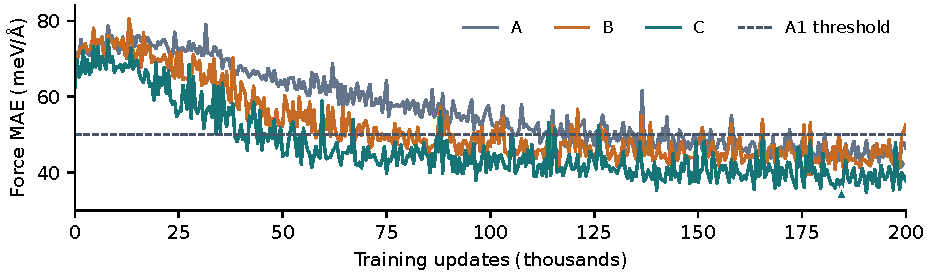
\includegraphics[width=\linewidth]{figures/baseline-curves.pdf}
\caption{Original energy-baseline validation trajectories, seed 0. Markers denote force-selected BEST checkpoints; the dashed line is the predeclared 50~meV/\AA\ adequacy threshold A1. Each point uses all 974 validation records and equal connection weighting.}\label{fig:baseline}
\end{figure}
C achieved 34.587~meV/\AA\ at update 184,500, compared with B's 40.370 and A's 42.108. It passed A1 and reduced the label-only zero-force reference of 62.504~meV/\AA\ by 44.664\%. Its force improvement over B comes with higher energy MAE, 126.990 versus 28.178~meV/molecule, at their separately force-selected checkpoints. A versus B changes both width and learning rate. These comparisons do not isolate width, fixed-update effects or cross-seed repeatability; selection and A1 use the same validation connections.

We then fixed C's recipe for nine subsequent fits: energy seed 1, two direct seeds and two seeds for each $\lambda\in\{0.1,1,10\}$. Reusing C seed 0 gives ten final-setting fits in total. Table~\ref{tab:prediction} reports both seed variation and the two-seed means.
\begin{table}[H]
\centering\small
\caption{Validation scores at force-selected BEST. The seed range is descriptive, not a confidence interval. Energy errors use the same saved checkpoints.}\label{tab:prediction}
\begin{tabular}{lrrr}\toprule
Formulation & Force MAE, mean & Seed min--max & Energy MAE, mean\\
 & \multicolumn{2}{c}{meV/\AA} & meV/molecule\\\midrule
Energy-derived & 34.893 & 34.587--35.198 & 128.725\\
Direct & 38.186 & 37.291--39.082 & 76.684\\
Consistency $\lambda=0.1$ & 38.024 & 36.773--39.275 & 87.006\\
Consistency $\lambda=1$ & 34.683 & 33.723--35.643 & 112.341\\
Consistency $\lambda=10$ & 39.725 & 39.060--40.390 & 161.662\\\bottomrule
\end{tabular}
\end{table}
BEST is optimistic because it minimizes 401 validation checks. Over updates 150,000--200,000, baseline trajectory standard deviations are 2.2--3.1~meV/\AA; these describe correlated training variation, not measurement uncertainty. In the nine subsequent fits, BEST is 0.1--7.4~meV/\AA\ below the final error. The 0.162~meV/\AA\ mean gap for $\lambda=0.1$ is much smaller than that variation, so matching is an operational rule rather than demonstrated equivalence.

Only $\lambda=0.1$ satisfies the original matching rule: the gap between two-seed mean force errors must be within 10\% of the smaller mean and within each arm's seed range. This matches aggregate means, not each seed individually. MACE Run A, trained for 2,048 epochs, has independently scored 5.349~meV/\AA\ equal-connection MAE (pooled MAE 5.260 reproduces the log; RMSE 26.410). Different architecture, training exposure and hardware make it an external reference, not a controlled efficiency comparison.
\begin{figure}[H]
\centering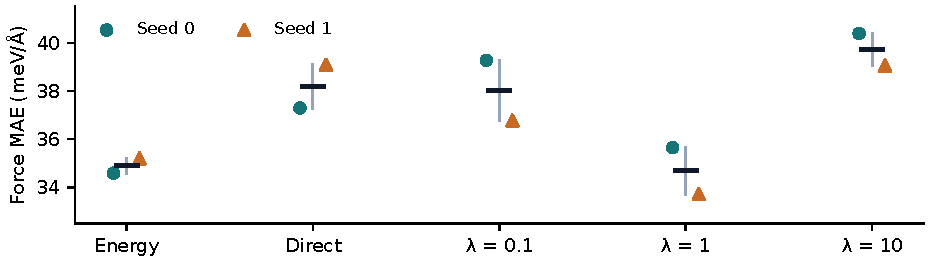
\includegraphics[width=\linewidth]{figures/controlled-force.pdf}
\caption{Validation force errors for two seeds per formulation. Ticks mark means; vertical lines join seed extrema, not confidence bounds. Two seeds do not establish superiority.}\label{fig:controlled}
\end{figure}
\section{Recovery failure and diagnosis}
The comparable predictive errors in Figure~\ref{fig:controlled} do not establish comparable recovery. Consistency strength 0.1 lowers normalized force/auxiliary-gradient disagreement MSE to 0.49--0.61 across seeds, versus 116--379 for direct prediction. However, its mean energy error is higher than direct prediction, and its observed fit-plus-score elapsed time is 1.985 times the direct arm's. This excludes separate diagnostics, earlier failures and unmeasured coordination overhead; it is not total project cost or inference speed. Better agreement on finite validation records does not establish global conservativity.

We evaluated five specific checkpoints: energy C seed 0, direct seeds 0/1 and matched-consistency seeds 0/1. Each starts from the same ten first stored branch frames across five validation connections, targeting six minima all seen in training. No-relaxation own-reference matching is 0/10; every model also recovers 0/10. The recovery pilot gate A2 fails. Across the 50 model/branch outcomes, 25 force-converged endpoints have wrong geometry and the other 25 do not converge. Reusing the same five connections across models does not create 50 independent observations.

The fixed procedure proposes $\mathbf R_{\mathrm{trial}}=\mathbf R+\eta\mathbf F$, initially $\eta=0.2$~\AA$^2$/eV. Accepted-step growth doubles $\eta$ up to 1.0; backtracking halves it, with a $10^{-8}$ floor and at most 40 trials. Each branch has 1,500 force attempts. Trial convergence is checked first; otherwise force agreement permits acceptance when $\mathbf F_{\mathrm{trial}}\cdot\mathbf F_{\mathrm{known}}\geq-10^{-12}$. There is no energy-decrease test. This caps scale, not displacement, despite inaccurate historical docstring wording. We retained the source and original results.
\begin{table}[H]
\centering\small
\caption{All models recover 0/10 original branches, whose six target classes are seen in training. Post-hoc reference-start controls use those classes and do not change A2.}
\begin{tabular}{lrr}\toprule
Checkpoint & Wrong converged / nonconverged & Reference-start recovery\\\midrule
Energy C seed 0 & 2 / 8 & 4/6\\
Direct seed 0 & 4 / 6 & 1/6\\
Direct seed 1 & 4 / 6 & 0/6\\
Consistency 0.1 seed 0 & 6 / 4 & 0/6\\
Consistency 0.1 seed 1 & 9 / 1 & 0/6\\\bottomrule
\end{tabular}
\end{table}
A 155-evaluation diagnostic reproduced all 50 stopping flags. Every model exceeded the force criterion at all 11 exact DFT minima, whose label forces remained below 2.745~meV/\AA. This does not rule out nearby points satisfying our tolerances. All 23 converged dual-head endpoints had disconnected 5~\AA\ neighbor graphs, so they are not intact molecular conformations. Beyond the cutoff, separated fragments exert no learned force on each other, although internal fragment forces may remain. Seven endpoints had every atom isolated: their direct force is automatically exactly zero. Both converged energy endpoints remained connected, but a separate nonconverged energy endpoint also separated.

Four selected traces reproduced saved endpoints exactly. Two separated, with largest accepted atom jumps of 436.721~\AA\ (direct) and 268.047~\AA\ (energy). The other two remained connected, with maxima 0.086492~\AA\ (consistency) and 0.006083~\AA\ (energy). These selected replays expose a procedure limitation, without proving sole causality, chemical dissociation or population rates.
\section{Discussion and remaining work}
All arms, including the energy baseline, fail the original pilot, leaving the comparative hypothesis unresolved beyond this procedure. Matching validation error and improving finite-record agreement did not produce recovery. Diagnostics identify coupled model/procedure limitations, not a penalty-specific cause. In the strict all-isolated limit of these E3x models, the consistency residual is uninformative; auxiliary gradients at the seven isolated endpoints were not measured.

Energy meets both endpoint criteria from 4/6 reference starts, versus at most 1/6 for either dual-head arm. This suggests limitations beyond the original starting geometries, without isolating a penalty effect. These 30 controls do not prove pathwise stability, exact stationary points or absence of nearby solutions.

Evidence covers aspirin, five validation connections and two seeds per formulation, with shared minima limiting independence. Validation selects both the recipe and BEST, so test generalization is unestablished. No stability, reaction-rate or barrier claim follows. MACE recovery remains unmeasured.
\paragraph{Changes from the proposal.}
The submitted proposal planned three seeds and a separate paracetamol replication. We have completed two seeds for the selected E3x settings; paracetamol remains deferred pending aspirin feasibility. Responsibilities have also been redistributed since the proposal. A revised adequacy protocol was adopted before the controlled comparison after unsuccessful small-subset checks; the original failures remain documented. Closed-loop, matched wall-time and complete inference-cost studies remain pending.
\paragraph{Three next actions.}
First, finish the MACE checkpoint loader and verify predictions against the saved validation outputs, then run the unchanged ten-start/six-reference procedure control. Second, use that control to decide whether a separately declared solver revision is justified; apply any revision to the same checkpoints and starts and label reused-validation analyses as post-hoc. Third, measure closed-loop work on preselected loops and batched prediction latency on identical hardware, then plan a fair wall-time comparison before final analysis and any one-time test evaluation. The first two controls reuse existing checkpoints; a new wall-time training comparison needs a separate budget.
\paragraph{Team roles and repository.}
Shedrack completed data preparation, model/training integration, the first MACE reference and current experiments. Olufunke authored the shared recovery evaluator. Emmanuel owns the remaining physical/cost analysis, and Idris owns MACE loading/admission and independent reproduction; these assignments are not completed-result claims. Members must confirm contributions before submission. Reviewed draft, code and evidence: \href{https://github.com/Shedrackeze002/idl-molecular-force-consistency/pull/10}{repository PR \#10} (stacked on PRs \#9 and \#8). The repository is private; staff access and an accessible reviewed revision must be confirmed before submission.
\begin{thebibliography}{5}\small
\bibitem{landscape} V. C\u{a}rare et al. Global properties of the energy landscape: a testing and training arena for machine learned potentials. \emph{npj Computational Materials}, 12:9, 2026. \href{https://doi.org/10.1038/s41524-025-01878-x}{doi:10.1038/s41524-025-01878-x}.
\bibitem{bigi} F. Bigi, M. F. Langer and M. Ceriotti. The dark side of the forces: assessing non-conservative force models for atomistic machine learning. \emph{ICML}, PMLR 267:4384--4414, 2025. \url{https://proceedings.mlr.press/v267/bigi25a.html}.
\bibitem{e3x} O. T. Unke and H. Maennel. E3x: E(3)-equivariant deep learning made easy. arXiv:2401.07595, 2024. \url{https://arxiv.org/abs/2401.07595}.
\bibitem{mace} I. Batatia et al. MACE: Higher order equivariant message passing neural networks for fast and accurate force fields. \emph{NeurIPS}, 35:11423--11436, 2022. \url{https://arxiv.org/abs/2206.07697}.
\bibitem{takamoto} M. Takamoto, V. Zaverkin and M. Niepert. Physics-informed weakly supervised learning for interatomic potentials. \emph{ICML}, PMLR 267:58282--58310, 2025. \url{https://proceedings.mlr.press/v267/takamoto25a.html}.
\end{thebibliography}
\end{document}
